A continuación se presenta un análisis comparativo de los tres métodos implementados.
Cabe mencionar que, dado que la experimentación requería que ambas imágenes (original y modificada) tengan el mismo tamaño para poder realizar un análisis cuantitativo de los algoritmos mediante las medidas de comparación que se mencionaron en la introducción, decidimos achicar la imagen original mediante un programa de edicion de imagenes para luego agrandarla mediante nuestros métodos y poder comparar los resultados obtenidos con la imagen original.

\subsection{Analisis de los metodos}

Empleamos un analisis incremental respecto al valor de los pixeles intermedios introducidos (el valor de $k$) para poder analizar los distintos metodos de forma escalonada y presentar conclusiones mucho mas claras. Dado que nuestros algoritmos solo funcionan cuando los valores de las imagenes son divisibles por $k$, no deben asumirse una correlacion entre los distintos valores de este debido a que las imagenes a analizar no siempre pudieron ser las mismas.

\subsubsection{K = 2}
Nuestro primer analisis se concentra en el valor minimo de $k$ para el cual esperabamos que el comportamiento de los tres metodos se mantenga bastante estable. Nuestra intuicion debenia de la idea de que todos ellos ofrecian una perdida en la calidad de la imagen bastanta pequ\~na en relacion al zoom que te estaba pidiendo.
Como podemos apreciar en los graficos a continuación, nuestra intuicion se corresponde con los valores de PSNR, donde los tres metodos se comportan relativamente iguales, sin embargo, nos sorprende ver que para el error cuadratico medio (y para PSNR tambien, pero en menor medida) la tecnica de interpolacion Bilineal obtuvo resultados muy destacables (de hecho, casi constantes), incluso frente a la tecnica de Splines que esperabamos siempre tenga un mejor rendimiento. La conclusion respecto de este fenomeno se explica al final del articulo.

\begin{center}
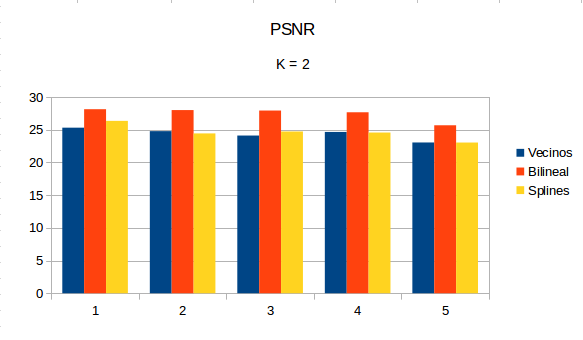
\includegraphics[scale=0.50]{imagenes/K2PSNR.png}
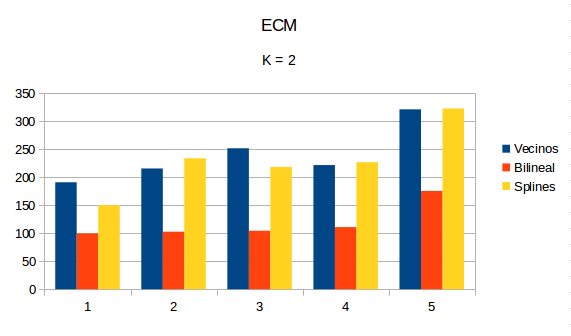
\includegraphics[scale=0.50]{imagenes/K2ECM.png}
\end{center}

\subsubsection{K = 4}
Para este segundo caso, es cierto que como esperabamos, el error cuadratico medio del metodo de los vecinos se dispara rapidamente mientras que los de interpiolacion bilineal y splines se mantienen practicamente iguales. Lo mismo sucede para los valores de PSNR, siendo los del metodo de vecinos los unicos que disminuyen con una diferencia de casi 5 puntos.

\begin{center}
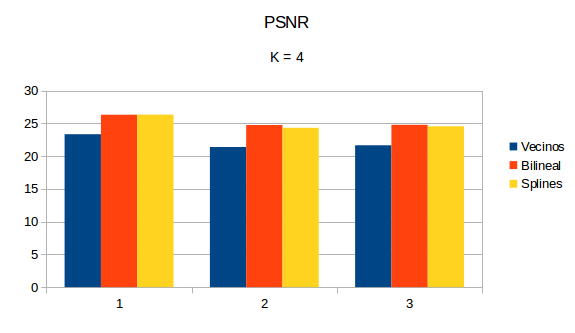
\includegraphics[scale=0.50]{imagenes/K4PSNR.png}
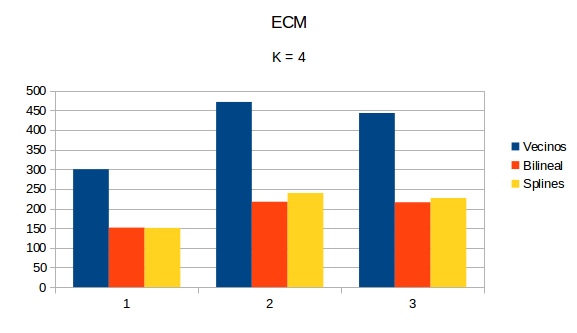
\includegraphics[scale=0.50]{imagenes/K4ECM.png}
\end{center}

\subsubsection{K = 6}
Entrando en valores de $k$ mucho mas elevados, nuestro analisis empezo a dejar de coincidir con lo que creiamos en un primer momento serian los resultados finales, debido a que el metodo de Splines no logro sacar una diferencia notoria frente al de interpolacion Bilineal sino que incluso, ambos metodos se mantuvieron practicamente constantes.  Al momento de obtener los resultados nos llamo poderosamente la atencion los valores de ECM obtenidos para las tres primeras imagenes, pero luego de hacer un analisis en conjunto de estas, llegamos a la conclusion de que la suba desmezurada en estos valores se debe a la elevada variabilidad de los contrastes en la escena (el interior de un hogar muy decorado, la foto aerea de un barrio, etc). 

\begin{center}
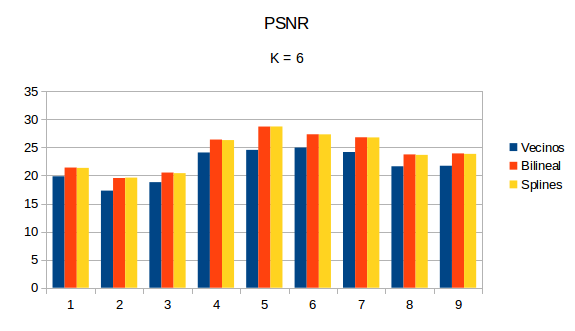
\includegraphics[scale=0.50]{imagenes/K6PSNR.png}
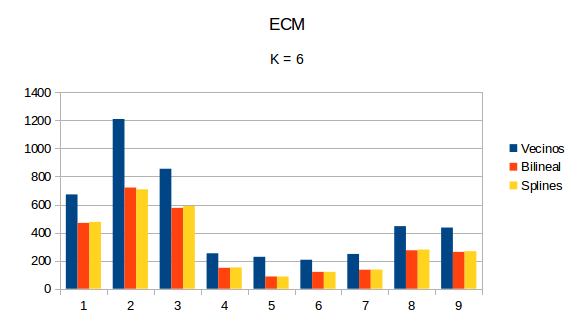
\includegraphics[scale=0.50]{imagenes/K6ECM.png}
\end{center}

\subsubsection{K = 10}
Por ultimo, para valores que ya se consiferan altos de $k$ el metodo de interpolacion Bilineal todavia sigue despe\~nandose igual o incluso a veces levemente mejor que el de Splines. Esto no solo contradice nuestra intuicion, sino que debido a la performance de ambos, estos resultados colocan al metodo de interpolacion como el mas apto en relacion benenficio/tiempo, muy por encima del de Splines (ambos ya muy por encima de el metodo de vecinos a esta altura).

\begin{center}
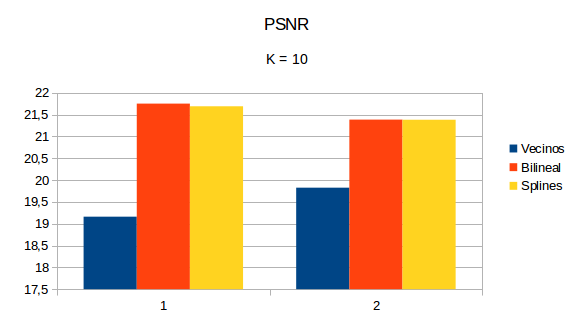
\includegraphics[scale=0.50]{imagenes/K10PSNR.png}
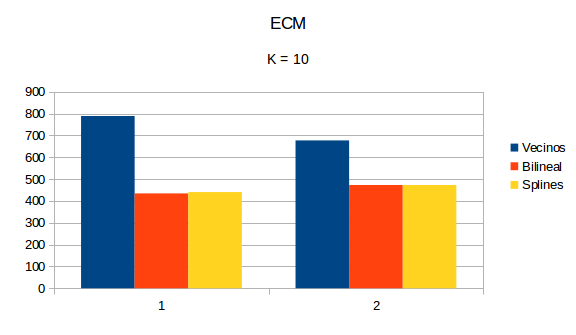
\includegraphics[scale=0.50]{imagenes/K10ECM.png}
\end{center}

\subsection{Analisis de tiempos}
El analisis de tiempo, a diferencia del de los metodos, no ofrecio ninguna respuesta que no hayamos podido intuir durante la codificacion de los algoritmos. Es claro que a medida que el metodo se perfecciona en la busqueda de resultados mas suaves, tambien aumenta el tiempo necesario de calculo.

\begin{center}
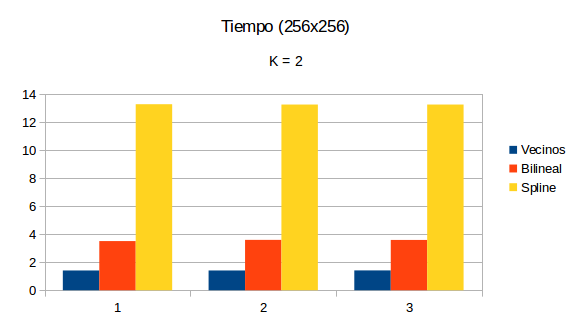
\includegraphics[scale=0.50]{imagenes/K2T1.png}
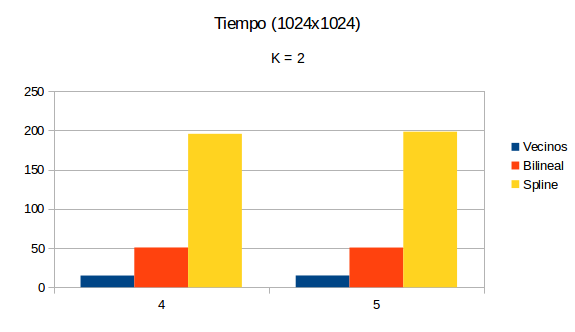
\includegraphics[scale=0.50]{imagenes/K2T2.png}
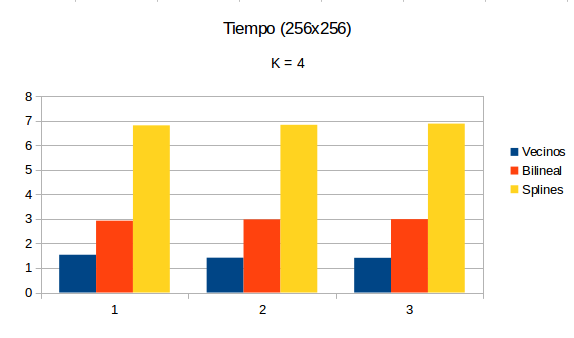
\includegraphics[scale=0.50]{imagenes/K4T.png}
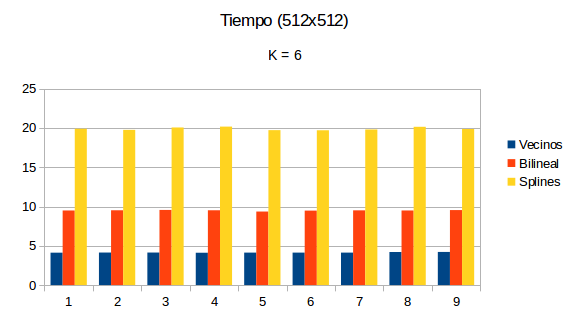
\includegraphics[scale=0.50]{imagenes/K6T.png}
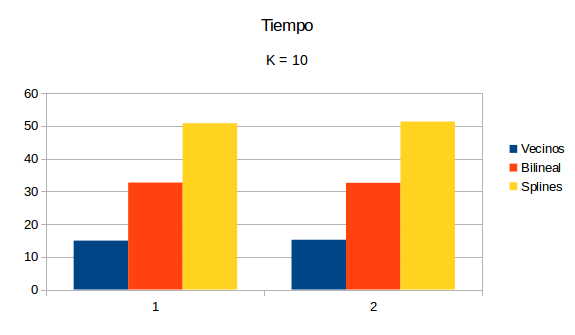
\includegraphics[scale=0.50]{imagenes/K10T.png}
\end{center}

